
%% bare_conf.tex
%% V1.3
%% 2007/01/11
%% by Michael Shell
%% See:
%% http://www.michaelshell.org/
%% for current contact information.
%%
%% This is a skeleton file demonstrating the use of IEEEtran.cls
%% (requires IEEEtran.cls version 1.7 or later) with an IEEE conference paper.
%%
%% Support sites:
%% http://www.michaelshell.org/tex/ieeetran/
%% http://www.ctan.org/tex-archive/macros/latex/contrib/IEEEtran/
%% and
%% http://www.ieee.org/

%%*************************************************************************
%% Legal Notice:
%% This code is offered as-is without any warranty either expressed or
%% implied; without even the implied warranty of MERCHANTABILITY or
%% FITNESS FOR A PARTICULAR PURPOSE! 
%% User assumes all risk.
%% In no event shall IEEE or any contributor to this code be liable for
%% any damages or losses, including, but not limited to, incidental,
%% consequential, or any other damages, resulting from the use or misuse
%% of any information contained here.
%%
%% All comments are the opinions of their respective authors and are not
%% necessarily endorsed by the IEEE.
%%
%% This work is distributed under the LaTeX Project Public License (LPPL)
%% ( http://www.latex-project.org/ ) version 1.3, and may be freely used,
%% distributed and modified. A copy of the LPPL, version 1.3, is included
%% in the base LaTeX documentation of all distributions of LaTeX released
%% 2003/12/01 or later.
%% Retain all contribution notices and credits.
%% ** Modified files should be clearly indicated as such, including  **
%% ** renaming them and changing author support contact information. **
%%
%% File list of work: IEEEtran.cls, IEEEtran_HOWTO.pdf, bare_adv.tex,
%%                    bare_conf.tex, bare_jrnl.tex, bare_jrnl_compsoc.tex
%%*************************************************************************

% *** Authors should verify (and, if needed, correct) their LaTeX system  ***
% *** with the testflow diagnostic prior to trusting their LaTeX platform ***
% *** with production work. IEEE's font choices can trigger bugs that do  ***
% *** not appear when using other class files.                            ***
% The testflow support page is at:
% http://www.michaelshell.org/tex/testflow/



% Note that the a4paper option is mainly intended so that authors in
% countries using A4 can easily print to A4 and see how their papers will
% look in print - the typesetting of the document will not typically be
% affected with changes in paper size (but the bottom and side margins will).
% Use the testflow package mentioned above to verify correct handling of
% both paper sizes by the user's LaTeX system.
%
% Also note that the "draftcls" or "draftclsnofoot", not "draft", option
% should be used if it is desired that the figures are to be displayed in
% draft mode.
%
\documentclass[12pt,conference]{IEEEtran}
% Add the compsoc option for Computer Society conferences.
%
% If IEEEtran.cls has not been installed into the LaTeX system files,
% manually specify the path to it like:
% \documentclass[conference]{../sty/IEEEtran}


\usepackage[margin=1in]{geometry}
\usepackage{listings}




% Some very useful LaTeX packages include:
% (uncomment the ones you want to load)


% *** MISC UTILITY PACKAGES ***
%
%\usepackage{ifpdf}
% Heiko Oberdiek's ifpdf.sty is very useful if you need conditional
% compilation based on whether the output is pdf or dvi.
% usage:
% \ifpdf
%   % pdf code
% \else
%   % dvi code
% \fi
% The latest version of ifpdf.sty can be obtained from:
% http://www.ctan.org/tex-archive/macros/latex/contrib/oberdiek/
% Also, note that IEEEtran.cls V1.7 and later provides a builtin
% \ifCLASSINFOpdf conditional that works the same way.
% When switching from latex to pdflatex and vice-versa, the compiler may
% have to be run twice to clear warning/error messages.






% *** CITATION PACKAGES ***
%
%\usepackage{cite}
% cite.sty was written by Donald Arseneau
% V1.6 and later of IEEEtran pre-defines the format of the cite.sty package
% \cite{} output to follow that of IEEE. Loading the cite package will
% result in citation numbers being automatically sorted and properly
% "compressed/ranged". e.g., [1], [9], [2], [7], [5], [6] without using
% cite.sty will become [1], [2], [5]--[7], [9] using cite.sty. cite.sty's
% \cite will automatically add leading space, if needed. Use cite.sty's
% noadjust option (cite.sty V3.8 and later) if you want to turn this off.
% cite.sty is already installed on most LaTeX systems. Be sure and use
% version 4.0 (2003-05-27) and later if using hyperref.sty. cite.sty does
% not currently provide for hyperlinked citations.
% The latest version can be obtained at:
% http://www.ctan.org/tex-archive/macros/latex/contrib/cite/
% The documentation is contained in the cite.sty file itself.






% *** GRAPHICS RELATED PACKAGES ***
%
\ifCLASSINFOpdf
   \usepackage[pdftex]{graphicx}
  % declare the path(s) where your graphic files are
  % \graphicspath{{../pdf/}{../jpeg/}}
  % and their extensions so you won't have to specify these with
  % every instance of \includegraphics
  % \DeclareGraphicsExtensions{.pdf,.jpeg,.png}
\else
  % or other class option (dvipsone, dvipdf, if not using dvips). graphicx
  % will default to the driver specified in the system graphics.cfg if no
  % driver is specified.
  % \usepackage[dvips]{graphicx}
  % declare the path(s) where your graphic files are
  % \graphicspath{{../eps/}}
  % and their extensions so you won't have to specify these with
  % every instance of \includegraphics
  % \DeclareGraphicsExtensions{.eps}
\fi
% graphicx was written by David Carlisle and Sebastian Rahtz. It is
% required if you want graphics, photos, etc. graphicx.sty is already
% installed on most LaTeX systems. The latest version and documentation can
% be obtained at: 
% http://www.ctan.org/tex-archive/macros/latex/required/graphics/
% Another good source of documentation is "Using Imported Graphics in
% LaTeX2e" by Keith Reckdahl which can be found as epslatex.ps or
% epslatex.pdf at: http://www.ctan.org/tex-archive/info/
%
% latex, and pdflatex in dvi mode, support graphics in encapsulated
% postscript (.eps) format. pdflatex in pdf mode supports graphics
% in .pdf, .jpeg, .png and .mps (metapost) formats. Users should ensure
% that all non-photo figures use a vector format (.eps, .pdf, .mps) and
% not a bitmapped formats (.jpeg, .png). IEEE frowns on bitmapped formats
% which can result in "jaggedy"/blurry rendering of lines and letters as
% well as large increases in file sizes.
%
% You can find documentation about the pdfTeX application at:
% http://www.tug.org/applications/pdftex





% *** MATH PACKAGES ***
%
%\usepackage[cmex10]{amsmath}
% A popular package from the American Mathematical Society that provides
% many useful and powerful commands for dealing with mathematics. If using
% it, be sure to load this package with the cmex10 option to ensure that
% only type 1 fonts will utilized at all point sizes. Without this option,
% it is possible that some math symbols, particularly those within
% footnotes, will be rendered in bitmap form which will result in a
% document that can not be IEEE Xplore compliant!
%
% Also, note that the amsmath package sets \interdisplaylinepenalty to 10000
% thus preventing page breaks from occurring within multiline equations. Use:
%\interdisplaylinepenalty=2500
% after loading amsmath to restore such page breaks as IEEEtran.cls normally
% does. amsmath.sty is already installed on most LaTeX systems. The latest
% version and documentation can be obtained at:
% http://www.ctan.org/tex-archive/macros/latex/required/amslatex/math/





% *** SPECIALIZED LIST PACKAGES ***
%
%\usepackage{algorithmic}
% algorithmic.sty was written by Peter Williams and Rogerio Brito.
% This package provides an algorithmic environment fo describing algorithms.
% You can use the algorithmic environment in-text or within a figure
% environment to provide for a floating algorithm. Do NOT use the algorithm
% floating environment provided by algorithm.sty (by the same authors) or
% algorithm2e.sty (by Christophe Fiorio) as IEEE does not use dedicated
% algorithm float types and packages that provide these will not provide
% correct IEEE style captions. The latest version and documentation of
% algorithmic.sty can be obtained at:
% http://www.ctan.org/tex-archive/macros/latex/contrib/algorithms/
% There is also a support site at:
% http://algorithms.berlios.de/index.html
% Also of interest may be the (relatively newer and more customizable)
% algorithmicx.sty package by Szasz Janos:
% http://www.ctan.org/tex-archive/macros/latex/contrib/algorithmicx/




% *** ALIGNMENT PACKAGES ***
%
%\usepackage{array}
% Frank Mittelbach's and David Carlisle's array.sty patches and improves
% the standard LaTeX2e array and tabular environments to provide better
% appearance and additional user controls. As the default LaTeX2e table
% generation code is lacking to the point of almost being broken with
% respect to the quality of the end results, all users are strongly
% advised to use an enhanced (at the very least that provided by array.sty)
% set of table tools. array.sty is already installed on most systems. The
% latest version and documentation can be obtained at:
% http://www.ctan.org/tex-archive/macros/latex/required/tools/


%\usepackage{mdwmath}
%\usepackage{mdwtab}
% Also highly recommended is Mark Wooding's extremely powerful MDW tools,
% especially mdwmath.sty and mdwtab.sty which are used to format equations
% and tables, respectively. The MDWtools set is already installed on most
% LaTeX systems. The lastest version and documentation is available at:
% http://www.ctan.org/tex-archive/macros/latex/contrib/mdwtools/


% IEEEtran contains the IEEEeqnarray family of commands that can be used to
% generate multiline equations as well as matrices, tables, etc., of high
% quality.


%\usepackage{eqparbox}
% Also of notable interest is Scott Pakin's eqparbox package for creating
% (automatically sized) equal width boxes - aka "natural width parboxes".
% Available at:
% http://www.ctan.org/tex-archive/macros/latex/contrib/eqparbox/





% *** SUBFIGURE PACKAGES ***
%\usepackage[tight,footnotesize]{subfigure}
% subfigure.sty was written by Steven Douglas Cochran. This package makes it
% easy to put subfigures in your figures. e.g., "Figure 1a and 1b". For IEEE
% work, it is a good idea to load it with the tight package option to reduce
% the amount of white space around the subfigures. subfigure.sty is already
% installed on most LaTeX systems. The latest version and documentation can
% be obtained at:
% http://www.ctan.org/tex-archive/obsolete/macros/latex/contrib/subfigure/
% subfigure.sty has been superceeded by subfig.sty.



%\usepackage[caption=false]{caption}
%\usepackage[font=footnotesize]{subfig}
% subfig.sty, also written by Steven Douglas Cochran, is the modern
% replacement for subfigure.sty. However, subfig.sty requires and
% automatically loads Axel Sommerfeldt's caption.sty which will override
% IEEEtran.cls handling of captions and this will result in nonIEEE style
% figure/table captions. To prevent this problem, be sure and preload
% caption.sty with its "caption=false" package option. This is will preserve
% IEEEtran.cls handing of captions. Version 1.3 (2005/06/28) and later 
% (recommended due to many improvements over 1.2) of subfig.sty supports
% the caption=false option directly:
%\usepackage[caption=false,font=footnotesize]{subfig}
%
% The latest version and documentation can be obtained at:
% http://www.ctan.org/tex-archive/macros/latex/contrib/subfig/
% The latest version and documentation of caption.sty can be obtained at:
% http://www.ctan.org/tex-archive/macros/latex/contrib/caption/




% *** FLOAT PACKAGES ***
%
%\usepackage{fixltx2e}
% fixltx2e, the successor to the earlier fix2col.sty, was written by
% Frank Mittelbach and David Carlisle. This package corrects a few problems
% in the LaTeX2e kernel, the most notable of which is that in current
% LaTeX2e releases, the ordering of single and double column floats is not
% guaranteed to be preserved. Thus, an unpatched LaTeX2e can allow a
% single column figure to be placed prior to an earlier double column
% figure. The latest version and documentation can be found at:
% http://www.ctan.org/tex-archive/macros/latex/base/



%\usepackage{stfloats}
% stfloats.sty was written by Sigitas Tolusis. This package gives LaTeX2e
% the ability to do double column floats at the bottom of the page as well
% as the top. (e.g., "\begin{figure*}[!b]" is not normally possible in
% LaTeX2e). It also provides a command:
%\fnbelowfloat
% to enable the placement of footnotes below bottom floats (the standard
% LaTeX2e kernel puts them above bottom floats). This is an invasive package
% which rewrites many portions of the LaTeX2e float routines. It may not work
% with other packages that modify the LaTeX2e float routines. The latest
% version and documentation can be obtained at:
% http://www.ctan.org/tex-archive/macros/latex/contrib/sttools/
% Documentation is contained in the stfloats.sty comments as well as in the
% presfull.pdf file. Do not use the stfloats baselinefloat ability as IEEE
% does not allow \baselineskip to stretch. Authors submitting work to the
% IEEE should note that IEEE rarely uses double column equations and
% that authors should try to avoid such use. Do not be tempted to use the
% cuted.sty or midfloat.sty packages (also by Sigitas Tolusis) as IEEE does
% not format its papers in such ways.





% *** PDF, URL AND HYPERLINK PACKAGES ***
%
%\usepackage{url}
% url.sty was written by Donald Arseneau. It provides better support for
% handling and breaking URLs. url.sty is already installed on most LaTeX
% systems. The latest version can be obtained at:
% http://www.ctan.org/tex-archive/macros/latex/contrib/misc/
% Read the url.sty source comments for usage information. Basically,
% \url{my_url_here}.





% *** Do not adjust lengths that control margins, column widths, etc. ***
% *** Do not use packages that alter fonts (such as pslatex).         ***
% There should be no need to do such things with IEEEtran.cls V1.6 and later.
% (Unless specifically asked to do so by the journal or conference you plan
% to submit to, of course. )


% correct bad hyphenation here
\hyphenation{op-tical net-works semi-conduc-tor}


\begin{document}
%
% paper title
% can use linebreaks \\ within to get better formatting as desired
\title{Consistency Guarantees}


% author names and affiliations
% use a multiple column layout for up to three different
% affiliations
\author{\IEEEauthorblockN{Michael Ben-Ami}
\IEEEauthorblockA{Columbia University\\
mzb2106@columbia.edu}
\and
\IEEEauthorblockN{Mateus Braga}
\IEEEauthorblockA{Columbia University\\
ma3382@columbia.edu}}

% conference papers do not typically use \thanks and this command
% is locked out in conference mode. If really needed, such as for
% the acknowledgment of grants, issue a \IEEEoverridecommandlockouts
% after \documentclass

% for over three affiliations, or if they all won't fit within the width
% of the page, use this alternative format:
% 
%\author{\IEEEauthorblockN{Michael Shell\IEEEauthorrefmark{1},
%Homer Simpson\IEEEauthorrefmark{2},
%James Kirk\IEEEauthorrefmark{3}, 
%Montgomery Scott\IEEEauthorrefmark{3} and
%Eldon Tyrell\IEEEauthorrefmark{4}}
%\IEEEauthorblockA{\IEEEauthorrefmark{1}School of Electrical and Computer Engineering\\
%Georgia Institute of Technology,
%Atlanta, Georgia 30332--0250\\ Email: see http://www.michaelshell.org/contact.html}
%\IEEEauthorblockA{\IEEEauthorrefmark{2}Twentieth Century Fox, Springfield, USA\\
%Email: homer@thesimpsons.com}
%\IEEEauthorblockA{\IEEEauthorrefmark{3}Starfleet Academy, San Francisco, California 96678-2391\\
%Telephone: (800) 555--1212, Fax: (888) 555--1212}
%\IEEEauthorblockA{\IEEEauthorrefmark{4}Tyrell Inc., 123 Replicant Street, Los Angeles, California 90210--4321}}




% use for special paper notices
%\IEEEspecialpapernotice{(Invited Paper)}




% make the title area
\maketitle


\begin{abstract}
%\boldmath
The abstract goes here.
\end{abstract}
% IEEEtran.cls defaults to using nonbold math in the Abstract.
% This preserves the distinction between vectors and scalars. However,
% if the conference you are submitting to favors bold math in the abstract,
% then you can use LaTeX's standard command \boldmath at the very start
% of the abstract to achieve this. Many IEEE journals/conferences frown on
% math in the abstract anyway.

% no keywords




% For peer review papers, you can put extra information on the cover
% page as needed:
% \ifCLASSOPTIONpeerreview
% \begin{center} \bfseries EDICS Category: 3-BBND \end{center}
% \fi
%
% For peerreview papers, this IEEEtran command inserts a page break and
% creates the second title. It will be ignored for other modes.
\IEEEpeerreviewmaketitle



\section{Introduction}
% no \IEEEPARstart

Our project is concerned with the subject of consistency in distributed systems, with a focus on etcd and its consistency guarantees in the middle of network partitions. Among the topics involved are consistency guarantees, verification and validation, network partitions, consensus and Jepsen, a framework to evaluate linearizability of distributed systems.

etcd is a consistent, key-store system that uses the Raft consensus algorithm and keeps fully available as long as there is a majority connected. Jepsen’s previous work has shown that etcd needed special care to deal with network partitions. In its latest version (v2.0), etcd has taken measures to make it clear what consistency guarantees are available. etcd provides two levels of consistency: sequential consistency and linearizability. We are interested in its linearizability guarantee, as it is the most intuitive consistency model to program against in a distributed setting. We reran the Jepsen tests on etcd for each of the two consistency levels.

A system, in its role of service provider, provides an interface to its users that performs a certain function. In the context of storage systems, memories, and databases, the system's high-level function is fundamental to programmers and involves in a way or another to remember data values for use in computation~\cite{saltzer2009principles}. Very different types of interfaces exist for such systems, for example, SQL, key-value mapping, file system, and objects, but all of them in a way or another allows for the user to read and write data. This project is interested in a particular property of storage systems: its consistency guarantees.

\section{Consistency}

Consistency can be a very confusing concept. Not only it has different meanings in different areas (database, system, and computer architecture communities), it interacts with other properties that themselves have different names (e.g. before-or-after atomicity and isolation). Nonetheless, consistency is an important concept that differentiates many storage system designs. 

The level of consistency of a storage system (its consistency guarantees) is an essential part of its function. In specific, it is about what values a read can return based on the order and the instant in time that the operations begin and end. Since it changes the meaning of read operations, an application -- as a user of the system -- would depend on a certain consistency guarantees to work correctly, hence the importance of studying and validating it.

A useful way to represent the function of a system, which includes its consistency guarantees, is through a model. A model of a system is intended to be simpler than its implementation, while still capturing the essential properties of the system. This is done by ignoring events that are not exposed through the system's interface. A fault tolerant distributed system model, for example, can be oblivious of data replicas and failure events tolerated by the implementation, since they are, by definition, not observed by the user~\cite{avizienis2004basic}. As with any other property in Computer Science, consistency can be formally expressed in terms of abstract algebra on top of a model. 'Survey on consistency conditions'~\cite{dziuma2013survey} does an excellent job as a formal presentation of the different major existing consistency guarantees. It comes from a computer architecture point of view but also surveys the consistency properties as they are used in the database community, including considerations like recoverability and avoiding cascading aborts.

Listing \ref{linearizableModelCode} shows the model of a linearizable register. It ignores any possible concurrency and failures that can occur in a real system while keeping the essential function of a linearizable register system. With such a model, it is possible to check whether a real execution trace could have been executed by a linearizable register system or not.

\begin{figure}[!t]
    \scriptsize
\begin{lstlisting}[caption={A Linearizable Register Model.},label={linearizableModelCode}]
=============================================
var currentValue

func handleOperation(operation) {
    switch (operation) {
    case ``read":
        return currentValue
    case ``write":
        currentValue = operation.value
    case ``CAS":
        if currentValue == operation.check {
            currentValue = operation.value
        }
    }
}
=============================================
\end{lstlisting}
\end{figure}

Consistency is a correctness property, and as such, needs to be always present in every execution of the system. This means it can be seen as a restriction on the possible history of events of the system (and its model). To say that a memory offers a certain consistency guarantee means that the memory system will never execute certain sequence of events made of reads and writes invocations and responses that does not pass the consistency conditions, as presented in~\cite{dziuma2013survey}. Consistency can also be extended to multi step operations, which can be seen as grouping of operations in transactions, and in this case its consistency conditions consider what transaction each event is part of.

\subsection{Why Different Levels of Consistency?}

The question of what value a read should return does not have one right answer, but usually an intuitive one. For a sequential process with its own private memory, the intuitive answer is that the read should return the last written value by the process. Todays programming model is not only concurrent, but also asynchronous and distributed. This reality requires considerations on what ``last written value" means, and brings the necessity of ordering operations in some way even in the absence of a global real-time clock. In order to do this, consistency models treat operations as an interval defined by the invocation and response point (on the invoker process). Another consequence of the asynchronous system reality is that performance and availability considerations brought an interest on weaker consistency models that fails on the intuition test, but attends applications that need the extra scalability.

The strongest practical consistency level is linearizability. It can be informally described as having each operation appear to have happen at a single point in time between invocation and the receipt of the response. By the definition, linearizability guarantees that every invocation in a sequential process will see the result of a previous one. It also guarantees that the process will see the result of any other operation that completed before its operation started. Finally, having the operations occur as a single point in time is essential for atomic conditional writes like check-and-set operations (CAS), which are building blocks for sophisticated abstractions like transactions. Unfortunately, as mentioned, all these guarantees are costly, and weaker consistency guarantees are also sought after.

Figure \ref{linearizabilityFigure} illustrates how the begin and end of the operations, along with its ``commit time" (the point in time which it appears to occur) puts restrictions on possible values returned in a read.

\begin{figure}[!t]
\centering
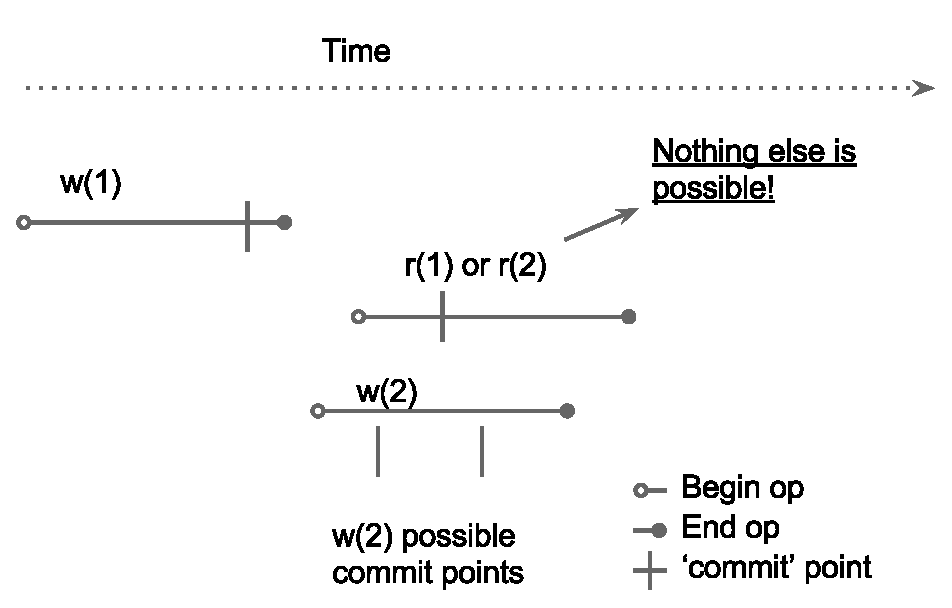
\includegraphics[width=3in]{images/linearizability}
\caption{Linearizability example.}
\label{linearizabilityFigure}
\end{figure}

The reason why an application can be OK with weaker consistency models is that what imposes requirements on the consistency model is the semantic of the data object being stored. An object for which any written value different than the initial default value is good enough (a semantical aspect) does not need linearizability. In fact, a replica that has seen a write does not need to be aware of any other write to the object. This allows for huge performance benefits. 

It is also possible to think how an application could have different consistency requirements for different data objects. Such application could make use of combinations storage systems consistency guarantees while paying in complexity costs. This is indicated on the formal definitions in~\cite{dziuma2013survey} as ``A sequential history H is legal, if for each object o, H | o belongs to the sequential specification for o."

Being able to work on stale data is related to whether conditional reads/writes (that is, reads/writes based on the value of an object) are critical to the correctness of the application. If missing a write is harmless for the function provided, many of the guarantees developed by years of research on storage systems can be left aside. Instead of the peace of mind of programming with the guarantee that transactions are atomic (as before-or-after and all-or-nothing properties), a weak consistency application might simply not have to worry about atomicity at all. So the ``problems" of weaker consistency might not be problems at all when it is appropriate for the application.

Even though there might be plenty of weak consistency applications out there, we have little experience with the design of such applications other than the potential use of causal consistency to support social network's link sharing, photos and albums dependencies~\cite{lloyd2011don}. We believe it is likely for applications to most of the time have a set of objects that requires linearizability, while others mostly-reads-and-rarely-updated objects could be separately stored in a weaker consistency (``cheaper") storage.

\section{Verification and Validation}

As a correctness criteria for the application, the consistency guarantees need to be well documented and enforced by the storage system. As shown by the Jepsen project~\cite{jepsenWebsite,jepsenGithubWebsite}, this is unfortunately not usually the case. Many popular databases fail to satisfy their consistency guarantees (in particular linearizability) when tested under realistic failure modes.

There are two methods to verify and validate a system's consistency guarantees. The first involves formally proving that the implementation design always satisfy the consistency model, in other words, it proves that by the design, it will never execute a sequence of events not allowed by the consistency model. Formal methods like this are usually not done in the industry and believed to require large amounts of time and hard to find expertise. Nevertheless, Amazon has reported successful stories of using TLA+~\cite{tlaWebsite}, a formal specification language, in the design and verification of its distributed storage systems~\cite{newcombe2014use}.

The second method is the test approach: find an execution that is not allowed by the consistency model. This method does not prove correctness if it does not find any incorrect execution, but can tell with certainty that the implementation is wrong when it finds one. A test approach requires a way to tell that an execution is incorrect. When verifying a system's consistency guarantee, this involves searching for a sequence of the events allowed by the model that is equivalent to the one produced by the real execution. This search space is huge and contains every possible order of the events observed concurrently by different users of the system. 

\subsection{Model Checking}

By answering whether an execution trace is acceptable in a consistency model, the test approach is effectively performing the job of a model checker for the context of consistency models. Since a model checker is also necessary in the formal methods approach, it is important to clarify the differences. 

In the test approach each execution trace is evaluated to see whether it is equivalent to a linearizable trace. Even though it can say for sure whether one particular execution trace conforms to the model, it can't say much about the other possible traces the system can execute. In a formal method approach, the design (not the implementation) is proved to always execute valid execution traces. Since the design still needs to be implemented, the formal method approach can't say for sure that an implementation implements the verified model either. \cite{newcombe2014use} argues that a formal proof is still worthwhile due to the increase in understanding of the design resulting from the formal proof specification process, and that this increases the chances of getting the code right.

\section{Jepsen/Knossos}

The Jepsen project~\cite{jepsenWebsite, jepsenGithubWebsite} is a test approach of evaluating a system's consistency guarantees. It provides a framework to execute tests on whether the database provides linearizability using read, write and CAS operations. At particular moments, Jepsen creates a network partition in the test environment. This is called the 'nemesis' process, and has the intention of stressing the system to increase the chance of finding bugs. By having clients record the execution trace of operations against the system, Jepsen can at the end of the execution analyze whether the trace is linearizable or not using the formal definition of linearizability~\cite{dziuma2013survey}.

Checking if a execution trace is linearizable is done by the Knossos part of the project. Its key idea uses the fact that in a linearizable schedule, each operation appears to occur at a single point in time. So it tries to find an ordering for all concurrent operations that is correct if executed in order by a single process ('correct by the model'). When trying the multitude of possible ordering, Knossos ignores any partial sequence in which is a violation of the model, pruning considerably the factorial search space by ignoring all sequences that contain an invalid prefix.~\cite{knossosPostWebsite}.

For example, if operation A cannot be before B, because A is a write(1) and B is a read(2), $A \rightarrow B \rightarrow C \rightarrow D$, and $A \rightarrow B \rightarrow D \rightarrow C$ cannot also be valid.

Knossos also makes use of others search techniques that includes parallelization, memoization, and priority queues. These techniques reduce the total number of histories of events that need to be explored by ignoring redundant histories (branches that arrives to an already visited state) and focusing on cheaper branches first~\cite{knossosPostWebsite2}.

For example, from the model in listing \ref{linearizableModelCode} it is easy to see that it does not matter how we got to a currentValue, since everything after that only cares about the current value. With this in mind, any two different branches in the search space that gets to the same state (current value), and still needs to consider the same set of operations, can be merged and we can be sure we will not miss anything.

\section{Network Partitions}

The CAP theorem points out that a system cannot provide both consistency and availability during network partitions. In other words, when a partition happens, which is inevitable, the system has to decide whether to return a potentially stale value for a read or refuse to process the request~\cite{brewer2012cap}. The CAP theorem referred to the linearizability consistency model but other works have shown that availability still conflicts with models as strong as sequential, serializable, repeatable read, snapshot isolation, or cursor stability consistency~\cite{strongConsistencyWebsite,bailis2013hat}. etcd uses the Raft consensus algorithm, and remains available as long as there is a majority connected. In case a partition separates the leader from the majority, a decrease in performance is observed by the clients for a short period of time due to a new leader being elected.

Network partitions do not necessarily affect the availability and consistency of the whole system. It depends on the scope of consistency (also called transaction unit) and scope of availability. The options are consistency (or availability) per register/shard/whole-storage~\cite{brewer2012cap}. etcd's transaction unit is the whole storage (enforced by Raft consensus), and should only be disabled when a majority is no longer connected. The other transaction units are related to data partitioning (also called sharding) but are not provided by etcd.

A system can discern when the partition ends by continuing to attempt communication~\cite{brewer2012cap}. etcd automatically resolves partitions (done by Raft consensus) but it requires manual intervention in case of majority partitions (also called a majority failure). This theoretically can be made automatic, but from the point of view of an operator something really bad is probably going on and would already require manual intervention anyway.

Client connection timeout should be treated as if the operation may or may not have completed. It does not mean the operation failed. Postgresql and Redis had this bug in 2013~\cite{postgresJepsenPostWebsite}. This matters because the consistency semantics are dependent on whether the operation succeeded or failed. Since etcd has a REST interface and client libraries, applications that uses the REST interface directly are responsible for doing this right, while the etcd client library should handle this for its users.

A partition between the service and the client only leaves the option for the client to work on disconnected operation and give up consistency~\cite{brewer2012cap}. This case is not analyzed in our project since etcd does not allow disconnected operation.

\section{etcd/Raft}

Raft is a consensus algorithm designed with understandability in mind. It provides a result equivalent to (multi)-Paxos, and it is as efficient as Paxos~\cite{ongaro2014search}. Its design includes leader election, snapshots, and membership changes. In Raft, the leader makes all the decisions regarding log entries and transmits them to the followers. Its election logic guarantees only one leader per ``term" and that any future leader will contain operations committed by previous leaders. Every new leader means a new term, in case where two leader is running, the one with the smaller term will become a follower as soon as it knows about the new leader.

etcd implements its consistency guarantees on top of the Raft consensus algorithm~\cite{ongaro2014search,etcdGithubWebsite}. It uses distributed consensus to answer what is the ``last written value" in a distributed setting. As Raft decides on an order to apply operations to a replicated state machine, the ``last written value" is chosen in its linearizability implementation by sending the read to the most current Raft leader, which returns the value of the last committed write. This guarantees linearizability because the most current Raft leader is the source of truth regarding which writes are committed at each point in time and no write response is sent before it is committed. 

etcd provides a choice on two consistency guarantees for the user's read requests. This is done in a per read request base with the quorum=true flag. A read with the quorum=true flag is guaranteed linearizability as explained above. The name of the flag comes from the necessary quorum of answers a raft leader needs to wait for in order to confirm it is the most current Raft leader. In a read with quorum=false (the default), the Raft leader does not ask for a confirmation to its peers that it is still the most current Raft leader. This option does not provide linearizability, and the value returned by the read might not be the last one committed. This happens when a new leader is elected and the previous leader that responded the read request does not know about it, so a write committed by the new leader would be ignored. 

It is possible for etcd to implement a leader lease to avoid a round-trip of a quorum for reads~\cite{gray1989leases}, similarly to Chubby~\cite{burrows2006chubby}, but as indicated in the Raft paper, this would rely on timing for safety since it assumes bounded clock skew~\cite{ongaro2014search}.

\section{Experiments}
\subsection {Environment}

The Jepsen software works by installing a desired distributed system on machines supplied by the user, and invoking reads and writes on it while creating network partitions. The machine on which Jepsen software runs will be referenced as the ``client machine". The user-supplied machines will be referenced as ``nodes".

Jepsen is written in Clojure, and so requires the leiningen~\cite{leiningen}, environment and a Java Virtual Machine (JVM) to be installed on the client machine.

The nodes do not have many requirements, except that they run the Debian operating system and that there are five of them~\cite{jepsenGithubWebsite}. In this way the nodes can be physical machines, virtual machines in a cloud environment, or even Linux containers. The software on the client machine communicates with the nodes over SSH and requires modification to the /etc/hosts file so that the Jepsen software can contact nodes by name. The SSH login credentials need to be hardcoded into the Jepsen source code. The nodes therefore need an SSH server installed and configured to accept root logins. The /etc/hosts file on the nodes themselves also needs to be configured with the same name-to-IP address mappings that client machine has. It is not necessary to manually install the desired distributed system on the nodes, as Jepsen automatically initiates downloads over SSH, installs all the required dependencies, and other tools needed for testing, like the iptables program. Jepsen uses iptables to simulate network partitions by installing blocking rules.

In our environment we rented a Linux VM from Amazon to act as the client machine, and set up Docker containers within the VM to act as the etcd nodes.

Jepsen comes prepackaged with the tools to test multiple distributed databases, including MongoDB, etcd, Aerospike, Consul, Elasticsearch, RabbitMQ, Cassandra, Zookeeper, NuoDB, and Kafka. However, Jepsen also provides an interface for a user to test any distributed database he wants by implementing certain methods in the source code. The user needs to implement setup() and teardown() methods for a custom database servers, and setup(), teardown(), and invoke() methods for clients transacting with those servers.

\subsection{Methodology}

Jepsen attempts to discover a non-linearizable history by simulating multiple clients, each one communicating with a different node in the etcd cluster, but all issuing multiple (around 90) random reads and writes to/from the same register in the span of about 30 seconds. Jepsen also introduces random network partitions during this time. Client invocations include read, write, and compare-and-set (CAS) operations. In response to these invocations, the clients may receive a response of ``ok'', indicating the requested operation was successful, ``fail", indicated the requested operation was unsuccessful, or ``info" indicating that it is unclear whether the requested operation was successful. The software keeps track on the client machine of what it expects to be in the register, and therefore which operations should be successful, and which values a read should return.

We used a ``random halves" partitioning that completely isolates two out of the five nodes from the other three. In this way there will always be a connected majority of three nodes, but it is indeterminate whether the current leader will be in that majority.

\subsection{Results}
We ran 10 tests with at both the ``default" and ``quorum=true" consistency levels. We found that at the default level of consistency, only 2 out of the 10 tests were linearizable in the presence of successive ``random halves" partitions. However, when under the ``quorum=true" consistency level, all 10 tests were successful in that they failed to produce a history that was not linearizable, even under the presence of random network partitions. Out of the 8 non-linearizable tests, 6 were failed due to an inconsistent read operation, and 2 failed due to an inconsistent CAS operation.

However, we also found that the ``quorum=true" setting, decreased availability during the tests. Under the default setting, no read operation timed out. But under the ``quorum=true" setting, 16\% of read operations timed out, on average. Both consistency settings exhibited timeouts for write and CAS operations at a rate or 20-25\%, on average.

\begin{figure}[!t]
\centering
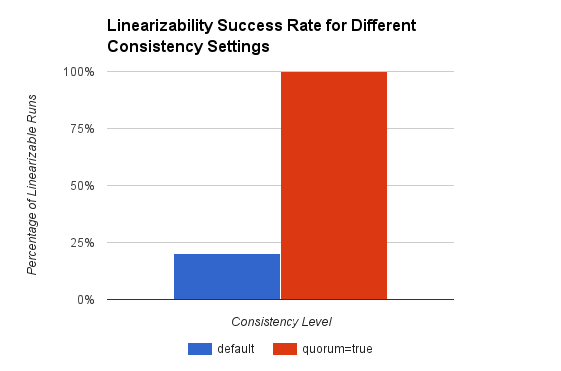
\includegraphics[width=3in]{images/overallresults}
\caption{Linearizability success rate for different consistency settings.}
\label{overallResultsFigure}
\end{figure}

\begin{figure}[!t]
\centering
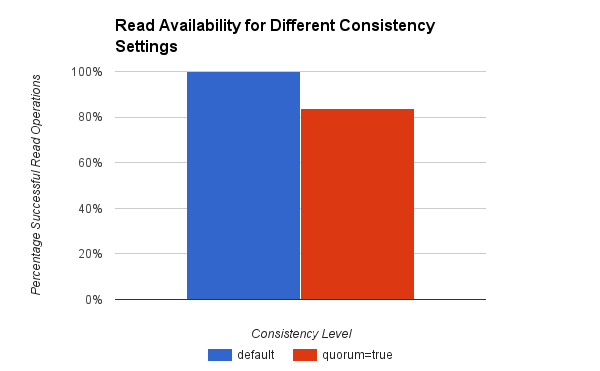
\includegraphics[width=3in]{images/availabilityresults}
\caption{Read availability for different consistency settings.}
\label{availabilityResultsFigure}
\end{figure}

\subsection{Interpreting Output}

Jepsen outputs a log to stdout while running tests. In this section we will examine some snapshots of the log and their meanings.

Listing 2 shows the log when Jepsen first starts up, indicated that five etcd nodes (labeled n1 through n5) are brought up and five ``workers" (virtual clients) are brought up to interact with those respective nodes.

\begin{figure}[!t]
    \scriptsize
\begin{lstlisting}[caption={Jepsen start sequence},label={jepsenStartSequence}]
=============================================
INFO  jepsen.system.etcd - :n1 starting etcd
INFO  jepsen.system.etcd - :n4 starting etcd
INFO  jepsen.system.etcd - :n3 starting etcd
INFO  jepsen.system.etcd - :n5 starting etcd
INFO  jepsen.system.etcd - :n2 starting etcd
INFO  jepsen.system.etcd - Running nodes: 
	{:n1 true, :n2 true,
	 :n3 true, :n4 true, :n5 true}
INFO  jepsen.system.etcd - :n3 etcd ready
INFO  jepsen.system.etcd - :n1 etcd ready
INFO  jepsen.system.etcd - :n4 etcd ready
INFO  jepsen.system.etcd - :n5 etcd ready
INFO  jepsen.system.etcd - :n2 etcd ready
INFO  jepsen.core - Worker 0 starting
INFO  jepsen.core - Worker 1 starting
INFO  jepsen.core - Worker 3 starting
INFO  jepsen.core - Worker 2 starting
INFO  jepsen.core - Worker 4 starting
=============================================
\end{lstlisting}
\end{figure}

Listing 3 shows the next phase of the Jepsen test, in which the virtual clients invoke database operations and receive responses. The number immediately following the hyphen represents the client process. Some operations succeed, and some fail. For example in Listing 3 we see that process 0 successfully writes the value ``3" to the register. Process 4 fails to do a CAS from ``2" to ``3". Presumably this is because 2 was not the current value of the register.

\begin{figure}[!t]
    \scriptsize
\begin{lstlisting}[caption={Jepsen Database Operations},label={jepsenTestingPhase}]
=============================================
INFO  jepsen.util - 0   :invoke :write  3
INFO  jepsen.util - 4   :invoke :cas    [2 3]
INFO  jepsen.util - 1   :invoke :write  3
INFO  jepsen.util - 0   :ok     :write  3
INFO  jepsen.util - 2   :ok     :cas    [3 1]
INFO  jepsen.util - 4   :fail   :cas    [2 3]
=============================================
\end{lstlisting}
\end{figure}

After some time, Jepsen introduces random network partitions. The output in Listing 4 represents nodes n1 and n5 becoming completely isolated from nodes n2, n3, and n4. In etcd, if the current leader is in the minority partition, a new leader election should take place.

\begin{figure}[!t]
    \scriptsize
\begin{lstlisting}[caption={Network Partition},label={networkPartition}]
=============================================
INFO  jepsen.util - :nemesis    :info   
	:start  ``Cut off {:n2 #{:n5 :n1}, :n4 #{:n5 :n1}, 
	:n3 #{:n5 :n1}, :n1 #{:n3 :n4 :n2}, 
	:n5 #{:n3 :n4 :n2}}"
=============================================
\end{lstlisting}
\end{figure}

When the operations and network partitions finish, the Knossos subsystem searches over the space of possibly linearizable histories. If it can't find one, it reports an inconsistent operation. Listing 5 shows that one of the read operations successfully read the value of ``4" from the register, when all histories indicate the value was ``0". Listing 6 shows one possible history (of many) that creates these circumstances.

\begin{figure}[!t]
    \scriptsize
\begin{lstlisting}[caption={Failure Result},label={failureResult}]
=============================================
Inconsistent state transitions:
([{:value 0} ``can't read 4 from register 0"])
=============================================
\end{lstlisting}
\end{figure}

\begin{figure}[!t]
    \scriptsize
\begin{lstlisting}[caption={Non-linearizable History},label={nlHistory}]
=============================================
World with fixed history:
3       :invoke :read   nil
1       :invoke :write  3
2       :invoke :cas    [3 1]
0       :invoke :write  3
3       :invoke :write  1
4       :invoke :write  0
1       :invoke :read   0
0       :invoke :write  0
3       :invoke :write  2
2       :invoke :write  4
3       :invoke :write  2
1       :invoke :read   2
0       :invoke :read   2
4       :invoke :write  3
3       :invoke :write  4
0       :invoke :read   4
1       :invoke :read   4
3       :invoke :write  0

led to state:
{:value 0}
=============================================
\end{lstlisting}
\end{figure}

\subsection{Analysis of Results}

We are not absolutely certain of what causes the inconsistent operations. However some prior work\cite{jepsenetcd} has been done in this area and suggests that when a network partition leaves a leader in the minority partition, a new leader election takes place in the majority, so there are two leaders on either side of the partition. The system has a ``split-brain". Under the default consistency level, reads are required to go through the leader. If the leader in the minority partition receives a read request before it is aware of the network partition, it will return the value in the register because it believes it is still the leader. The ``quorum=true" consistency level forces reads to go through the same raft consensus process as writes. This explains why there are no inconsistencies when under ``quorume=true", but also why availability decreases under this setting.

\section{Future Work}

We measured the effect of network partitions on availability under different consistency levels by recording the number of timed out operations. However, there is a richer set of availability measurements that can be gathered by examining latency statistics. Jepsen source code actually comes with the ability to gather latency measurements and output graphical results, but we could not figure out how to activate it in the scope of this semester.

Our tests partitioned the nodes into ``random halves". There are also different types of network partitions and network problems that can occur, and Jepsen's source code includes the ability to perform many of them. They include ``bridge" (a single node forms the path between two partitions), ``isolate" (isolates a single node from the cluster), ``clock scrambler" (randomly alters the system clock on each node), and ``asymmetric partitions" (traffic is allowed to flow in only one direction between partitions).

Our tests focused on etcd. However, there are many distributed systems that Jepsen supports, and many others that can be added as custom modules. Previous work has exposed specific failure conditions for specific systems. As far as we can see, there has been no work to run a collection of tests in bulk across different systems varying parameters (e.g. type of network partition), and comparing the results. It would be useful not only to compare whether the systems are linearizable, but the availability tradeoffs under different consistency settings. In fact, this was the original goal of the project, but we had some difficulty with the tools that prevented us from pursuing it in the scope of the semester.


% An example of a floating figure using the graphicx package.
% Note that \label must occur AFTER (or within) \caption.
% For figures, \caption should occur after the \includegraphics.
% Note that IEEEtran v1.7 and later has special internal code that
% is designed to preserve the operation of \label within \caption
% even when the captionsoff option is in effect. However, because
% of issues like this, it may be the safest practice to put all your
% \label just after \caption rather than within \caption{}.
%
% Reminder: the "draftcls" or "draftclsnofoot", not "draft", class
% option should be used if it is desired that the figures are to be
% displayed while in draft mode.
%
%\begin{figure}[!t]
%\centering
%\includegraphics[width=2.5in]{myfigure}
% where an .eps filename suffix will be assumed under latex, 
% and a .pdf suffix will be assumed for pdflatex; or what has been declared
% via \DeclareGraphicsExtensions.
%\caption{Simulation Results}
%\label{fig_sim}
%\end{figure}

% Note that IEEE typically puts floats only at the top, even when this
% results in a large percentage of a column being occupied by floats.


% An example of a double column floating figure using two subfigures.
% (The subfig.sty package must be loaded for this to work.)
% The subfigure \label commands are set within each subfloat command, the
% \label for the overall figure must come after \caption.
% \hfil must be used as a separator to get equal spacing.
% The subfigure.sty package works much the same way, except \subfigure is
% used instead of \subfloat.
%
%\begin{figure*}[!t]
%\centerline{\subfloat[Case I]\includegraphics[width=2.5in]{subfigcase1}%
%\label{fig_first_case}}
%\hfil
%\subfloat[Case II]{\includegraphics[width=2.5in]{subfigcase2}%
%\label{fig_second_case}}}
%\caption{Simulation results}
%\label{fig_sim}
%\end{figure*}
%
% Note that often IEEE papers with subfigures do not employ subfigure
% captions (using the optional argument to \subfloat), but instead will
% reference/describe all of them (a), (b), etc., within the main caption.


% An example of a floating table. Note that, for IEEE style tables, the 
% \caption command should come BEFORE the table. Table text will default to
% \footnotesize as IEEE normally uses this smaller font for tables.
% The \label must come after \caption as always.
%
%\begin{table}[!t]
%% increase table row spacing, adjust to taste
%\renewcommand{\arraystretch}{1.3}
% if using array.sty, it might be a good idea to tweak the value of
% \extrarowheight as needed to properly center the text within the cells
%\caption{An Example of a Table}
%\label{table_example}
%\centering
%% Some packages, such as MDW tools, offer better commands for making tables
%% than the plain LaTeX2e tabular which is used here.
%\begin{tabular}{|c||c|}
%\hline
%One & Two\\
%\hline
%Three & Four\\
%\hline
%\end{tabular}
%\end{table}


% Note that IEEE does not put floats in the very first column - or typically
% anywhere on the first page for that matter. Also, in-text middle ("here")
% positioning is not used. Most IEEE journals/conferences use top floats
% exclusively. Note that, LaTeX2e, unlike IEEE journals/conferences, places
% footnotes above bottom floats. This can be corrected via the \fnbelowfloat
% command of the stfloats package.



\section{Conclusion}

We presented a study of consistency in distributed database systems, and the effects of network partitions efcd's fulfillment of consistency guarantees. We found evidence to support that etcd fulfills its promises, and that higher consistency levels bring a tradeoff in availability. We offered a proposed explanation of what happens ``behind the scenes" when failures in linearizability happen. Finally, we proposed topics for future work in this area.



% conference papers do not normally have an appendix


% use section* for acknowledgement
\section*{Acknowledgment}

We would like to thank Professor Roxana Geambasu and her Teaching Assistants for an exciting and educational course on distributed systems. We would also like to thank Kyle Kingsbury, the author of the Jepsen project.





% trigger a \newpage just before the given reference
% number - used to balance the columns on the last page
% adjust value as needed - may need to be readjusted if
% the document is modified later
%\IEEEtriggeratref{8}
% The "triggered" command can be changed if desired:
%\IEEEtriggercmd{\enlargethispage{-5in}}

% references section

% can use a bibliography generated by BibTeX as a .bbl file
% BibTeX documentation can be easily obtained at:
% http://www.ctan.org/tex-archive/biblio/bibtex/contrib/doc/
% The IEEEtran BibTeX style support page is at:
% http://www.michaelshell.org/tex/ieeetran/bibtex/
%\bibliographystyle{IEEEtran}
% argument is your BibTeX string definitions and bibliography database(s)
\bibliographystyle{./IEEEtran}
\bibliography{./IEEEabrv,./report}
%
% <OR> manually copy in the resultant .bbl file
% set second argument of \begin to the number of references
% (used to reserve space for the reference number labels box)
%\begin{thebibliography}{1}
%
%\bibitem{IEEEhowto:kopka}
%H.~Kopka and P.~W. Daly, \emph{A Guide to \LaTeX}, 3rd~ed.\hskip 1em plus
  %0.5em minus 0.4em\relax Harlow, England: Addison-Wesley, 1999.
%
%\end{thebibliography}






% that's all folks
\end{document}
